\usecasebase{Visualizzazione notifica stato della prenotazione}
\label{usecase:Visualizzazione notifica stato della prenotazione}

\begin{figure}[h]
	\centering
	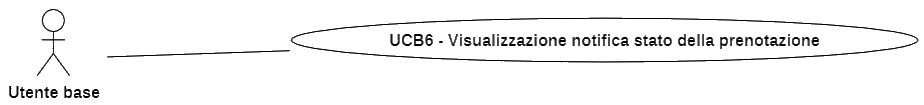
\includegraphics[width=0.9\textwidth]{./uml/UCB6.png} 
	\caption{Visualizzazione notifica stato della prenotazione}
	\label{fig:UCB6}
  \end{figure}

\begin{itemize}
	\item \textbf{Attore principale:} Utente base.

	\item \textbf{Precondizione:} L'Utente ristoratore ha cambiato lo stato della prenotazione (vedi \autoref{usecase:Accetta prenotazione},
	      \autoref{usecase:Rifiuta prenotazione} e \autoref{usecase:Termina prenotazione}).


	\item \textbf{Postcondizione:} L'Utente base visualizza la notifica del cambiamento di stato della sua prenotazione.

	\item \textbf{Scenario principale:}
	      \begin{enumerate}
		      \item Il Sistema rivela un cambiamento dello stato della prenotazione;
		      \item Il Sistema invia agli Utenti base relativi a questa
		            prenotazione una notifica sul cambio dello stato;
		      \item L'Utente base visualizza la notifica del cambiamento di stato della sua prenotazione, la quale si può trovare in:
		            \begin{itemize}
			            \item Accettata dall'Utente ristoratore.
			            \item Rifiutata dall'Utente ristoratore (con le motivazioni del rifiuto).
			            \item Terminata dall'Utente ristoratore.
		            \end{itemize}
	      \end{enumerate}
\end{itemize}
